\documentclass[10pt, conference, compsocconf]{IEEEtran}
\IEEEoverridecommandlockouts

\usepackage{float}
\usepackage{cite}
\usepackage[pdftex]{graphicx}
\usepackage{amstext,epsfig,amssymb,amsbsy,amsthm}
\usepackage{algorithmic}
\usepackage{array}
\usepackage{color}
\usepackage{graphicx}
\usepackage{mathtools}
\graphicspath{ {./figures/} }
\usepackage{amsfonts}
\usepackage{bm}
\usepackage{soul}
\usepackage{dblfloatfix} % fix for bottom-placement of figure
\usepackage{tikz, pgfplots} % Necessary package for tikz
\usepgfplotslibrary{groupplots}
\usetikzlibrary{pgfplots.groupplots}
\pgfplotsset{ % Here we specify options for all figures in the document
colorbar shift/.style={xshift=-1mm},
colorbar/width = .3cm,
every axis label/.append style={font=\scriptsize},
every y axis label /.append style={xshift=3mm},
every tick label/.append style={font=\scriptsize},
every colorbar/.append style={
        yticklabel style={
            text width=1em,
	font=\scriptsize,
            align=left,
	baseline}},
every axis title/.append style={font=\scriptsize, yshift=-2mm, overlay},
compat=1.3,
}
\usetikzlibrary{calc}
\usepackage{amsmath,amssymb}
\usepackage{subcaption}
\usepackage{nomencl} 
\makenomenclature
\allowdisplaybreaks[3]

\newtheorem{theorem}{Theorem}
\newtheorem{lemma}{Lemma}
\newtheorem{corollary}{Corollary}
\newtheorem{proposition}{Proposition}
\theoremstyle{definition}
\newtheorem{remark}{Remark}

\newcommand{\rank}{{\textrm rank}}
\newcommand{\by}{\mathbf{y}}
\newcommand{\bx}{\mathbf{x}}
\newcommand{\bX}{\mathbf{X}}
\newcommand{\bP}{\mathbf{P}}
\newcommand{\bp}{\mathbf{p}}
\newcommand{\bv}{\mathbf{v}}
\newcommand{\bs}{\mathbf{s}}
\newcommand{\bS}{\mathbf{S}}
\newcommand{\bq}{\mathbf{q}}
\newcommand{\bi}{\mathbf{i}}
\newcommand{\br}{\mathbf{r}}
\newcommand{\bQ}{\mathbf{Q}}
\newcommand{\bI}{\mathbf{I}}
\newcommand{\bM}{\mathbf{M}}
\newcommand{\be}{\mathbf{e}}
\newcommand{\bl}{\bm{\ell}}

\newcommand{\bw}{\mathbf{w}}
\newcommand{\bW}{\mathbf{W}}
\newcommand{\bu}{\mathbf{u}}
\newcommand{\bb}{\mathbf{b}}

\newcommand{\bZ}{\mathbf{Z}}
\newcommand{\bV}{\mathbf{V}}
\newcommand{\bA}{\mathbf{A}}
\newcommand{\bB}{\mathbf{B}}
\newcommand{\bC}{\mathbf{C}}
\newcommand{\bD}{\mathbf{D}}
\newcommand{\bn}{\mathbf{n}}
\newcommand{\bY}{\mathbf{Y}}
\newcommand{\eye}{{\rm j\;}}
\newcommand{\bDelta}{\boldsymbol{\Delta}}
\newcommand{\re}{{\rm Re}}
\newcommand{\im}{{\rm Im}}
\newcommand{\Tr}{\textrm{Tr}}
\newcommand{\Vect}{\textrm{vec}}
\newcommand{\prob}{\textrm{prob}}
\newcommand{\1}{1{\hskip -2.55 pt}\hbox{I}}
%%%%%%%%%%%%%%%%%%%%%%%%%%%
% calligraphic symbols
%%%%%%%%%%%%%%%%%%%%%%%%%%%
\DeclareMathOperator*{\argmax}{arg\,max}
\DeclareMathOperator*{\argmin}{arg\,min}

\newcommand{\co}{\textrm{co}}
\newcommand{\cgend}{\mathscr{C}^\textrm{gen}_{\textrm{dyn}}}
\newcommand{\cgens}{\mathscr{C}^\textrm{gen}_{\textrm{stat}}}
\newcommand{\pg}[2]{p_{g_{#1}}^{#2}}
\newcommand{\qg}[2]{q_{g_{#1}}^{#2}}
\newcommand{\ug}[2]{u_{g_{#1}}^{#2}}
\newcommand{\cg}[2]{\check{u}_{g_{#1}}^{#2}}
\newcommand{\pw}[2]{\mathbf{p}_{r_{#1}}^{#2}}
\newcommand{\ld}[1]{\mathbf{L}^{#1}}
\newcommand{\ldk}[2]{\mathbf{L}^{#1}_{#2}}
\newcommand{\pgmax}[1]{p_{{g}_{\text{max},#1}}}
\newcommand{\pgmin}[1]{p_{{g}_{\text{min},#1}}}
\newcommand{\rup}[1]{R_{\text{up},#1}}
\newcommand{\rdn}[1]{R_{\text{dn},#1}}
\newcommand{\Prob}{\mathbb{P}}
\newcommand{\R}{\mathbb{R}}
\DeclareMathOperator*{\argminB}{argmin}
\DeclareMathOperator*{\argminC}{min}
\makenomenclature 

\begin{document}
\newlength\figureheight
\newlength\figurewidth
\title{}
\author{}

\maketitle

% -------------------------------------------------------------------------
% Abstract
% -------------------------------------------------------------------------
\begin{abstract}


\end{abstract}


\begin{IEEEkeywords}

\end{IEEEkeywords}
\IEEEpeerreviewmaketitle
\printnomenclature
%\section{Introduction}\label{sec:Intro}
%%!TEX root = HICSS51.tex
With the advance in smart grid technologies, the electricity market has been transforming from a centralized market to a deregulated market, from a vertical structure to a horizontal structure due to some driving factors such as renewable generation, demand response and distributed generation \cite{nesamalar2016energy}. Consequently, the market is becoming more dynamic and competitive \cite{sun2017identifying}. To suit this deregulated market nature, it is paramount for the three main players in the market namely generation, transmission and distribution to optimize their operation strategies by modeling the interactions between themselves and the other market players. This interaction could be essentially viewed from a game-theory perspective and could be modeled through some game structure. Specifically, bilevel optimization which is closely related to the Stackelberg game in economics is widely applied to model the interaction among the three players \cite{colson2007overview}. 

Bilevel optimization is defined as a mathematical optimization problem in which one optimization problem (upper level problem) contains another optimization problem (lower level problem) \cite{bilevel1}. There are two types of approaches to solve bilevel optimization problems. The first category applies classical methods including single-level reduction \cite{bialas1984two,bard1982explicit}, descent \cite{kolstad1990derivative,savard1994steepest}, penalty function \cite{lv2007penalty,white1993penalty}, and trust-region methods \cite{colson2005trust,marcotte2001trust}. Most of the classical approaches deal with convex problems. Some strong assumptions such as continuous differentiability and lower semi-continuity are also quite common. Of those methods, single level reduction is the most widely used one when the lower level problem is convex. The single level reduction method is applied in this work. The second category applies evolutionary methods including genetic algorithms \cite{mathieu1994genetic}, particle swarm optimization \cite{li2006hierarchical}, differential evolution \cite{zhu2006hybrid}, and metamodeling-based methods \cite{wang2007review}. They normally require significant computational efforts and may not perform well. For a detailed review of different bilevel optimization methods, please refer to \cite{bilevel1, bilevel2}. 

There has been on-going research of bilevel optimization of in the power systems. In \cite{vahidinasab2009multiobjective,soleymani2008new,kozanidis2013mixed,zhang2011competitive,andrianesis2011mixed}, the bidding strategies of generation companys(Genco) are studied, in which the Genco's payoff is formulated as the upper level problem and the independent system operator's dispatch is formulated as the lower level problem. The planning and investment of different power system components using a bilevel optimization framework is investigated in \cite{verma2018information, zolfaghari2018bilevel, pandvzic2018investments, zhou2011designing, baringo2011wind}. \cite{yuan2011modeling, xiang2017coordinated, arroyo2009genetic, pinar2010optimization,arroyo2010bilevel} use bilevel optimization to study power system vulnerability issues which focus on minimizing the system loss under terrorist attacks on some transmission line or generator. The bilevel optimization work closely related to our work which centers on the transmission and distribution interaction appears in \cite{haghighat2012bilevel, li2007multiperiod, zhang2016trading}. In those work,  the distribution system optimal dispatch is the upper level problem, while the transmission system optimal dispatch is the lower level problem.  In \cite{haghighat2012bilevel}, the author uses bilevel optimization for the operational decision making of a distribution company(DS) in a competitive market with many other DSs.  A multi-period energy acquisition bilevel optimization model is proposed for a distribution company with distributed generation(DG) and interruptible load(IL) in \cite{li2007multiperiod}. The roles of DG and IL to alleviate congestion are also analyzed in the bilevel framework.  Trading strategies of DSs with distributed energy resources are examined in the day-ahead market and real time market in \cite{zhang2016trading}. For those work, there is a main problem with having the DS as the upper level problem. The upper level problem needs to know the lower level problem information such as GENCO information as well as other DSs's information, however it is unrealistic to assume the DS has that information. It is more intuitive and reasonable to have the transmission system operated by the independent system operation(ISO) as the upper level problem and the DS as the lower level problem since the ISO receives information from both the GENCO side and DS side and the ISO is at the top level in the power system hierarchy.

Int this work, the ISO or transmission system dispatch is formulated as the upper level problem, the DSs are formulated as the lower level problem. Under this structure, the upper level problem decides the energy and demand response prices of the DSs, the lower level problem responds by deciding the quantity of DR and energy import. The key contributions of this work are summarized below.

1. Present a bilevel optimization framework for the transmission and distribution system co-optimization.

2. Compare the bilevel optimization approach with the traditional co-optimization approach in different aspects. 

3. Reformulate the bilevel problem as a single level problem with KKT conditions and linearize the resulting nonlinear problem with the big-M method and strong duality theorem.

The structure of the paper is as follows; the problem under study is described in section~\ref{sec:pd}, the bilevel optimization model is discussed in section~\ref{sec:Model}.  Numerical results for are reported in Section~\ref{sec:Results}. Concluding remarks and future research directions follow in Section~\ref{sec:Conclude}. 

\section{Problem Description}\label{sec:pd}
%!TEX root = HICSS51.tex
% conclusions

\subsection{Transmission System Problem}
The TS has a network of transmission lines and buses. Traditional and renewable generation units, loads and DS are connected to different buses in the network. The TS solves a day ahead market unit commitment problem, which is a co-optimization of the energy market and ancillary service market. For the energy market optimization, the TS tries to minimize the cost of meeting the system demand with its own generation or energy from DS. For the ancillary service market optimization, the TS minimizes the cost of providing enough reserve to account for the renewable forecast uncertainty. The reserve service could either come from the TS generator's reserve or the DS's DR. The TS objective function minimizes the energy and ancillary service cost at the same time.  

\subsection{Distribution System Problem}
The distribution system has dispatchable load and non-dispatchable load, and distributed generation in a radial network. In the day-ahead market, the DS solves an optimal dispatch problem with power flow. The dispatchable load is optimized at some point in between its upper and lower bound. The difference between the upper/lower bound and its set point could be used to provide upward/downward DR. The objective of the DS is to minimize the cost of meeting its demand either by its distributed generation or importing power from the TS and maximize the revenue of providing DR

\subsection{Co-operation Mode}
Under the bilevel co-optimization framework, the TS decides the price of DS energy import as well as the price for purchasing DS DR, the DS responds to those prices by exchanging a certain amount of energy with the TS and selling a certain amount of DR to the TS.

The co-optimization between the TS and DS is illustrated in Fig.~\ref{wees}
\begin{figure}
\centering
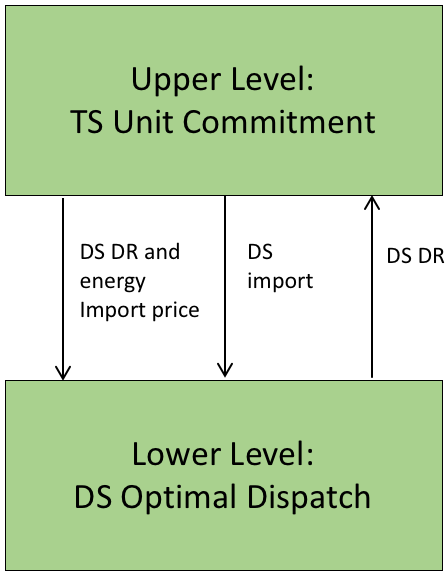
\includegraphics[scale=0.3]{flows.png}
\caption{Co-optimization between the TS and MG}
\label{wees}
\end{figure}

\subsection{Renewable Forecast Uncertainty Management}
In this work, we use a robust approach to manage the uncertainty in renewable forecast. Specifically, for a renewable generation forecast and a set of possible generation scenarios, we calculate the upward/downward forecast deviation by taking the difference of the hourly maximum/minimum generation scenario and the hourly forecast. The downward/upward TS generation reserve and upward/downward MG DR are used to account for the upward/downward renewable forecast deviation.


\section{Model Formulation}\label{sec:Model}
%!TEX root = HICSS51.tex
In this section, the structure of the bi-level optimization problem is described. The general formulation of a bilevel optimization is given below:

\begin{align}
\begin{aligned}
&\argminC_{x\in X, y\in Y}F\left(x,y\right) \\
\text{st:   }  & G_i\left(x,y\right)\leq 0, \text{for   }  i \in \{1,2,...,I\}\label{prime}\\
& H_k\left(x,y\right) = 0, \text{for   }  k \in \{1,2,...,K\}\\
& y\in \argminB_{y\in Y} \{f(x,y): g_j(x,y)\leq 0, \text{for   }  j \in \{1,2,...,J\}, \\ 
                                                   &h_m(x,y) = 0, \text{for   }  m \in \{1,2,...,M\}  \}
\end{aligned}
\end{align}


In the above formulation, $x,F(x,y),(G_i, H_k)$ are the optimization variables, objective function and constraints of the upper level problem. Whereas, $y,f(x,y),(g_i,h_m)$ are the optimization variables, objective function and constraints of the lower level problem. According to this formulation, the bilevel formulation of the TS and DS co-optimization is given in the following sections. 

\subsection{Upper Level Problem: TS Unit Commitment Problem}

The upper level transmission day-ahead unit commitment problem seeks to compute the optimal operation schedule including the generator commitment status $w_{g,t}$, generation output $p_{g,t}$, upward and downward generator's reserve $R^{up}_{g,t}$, $R^{dn}_{g,t}$, DS DR price $P^{dr}_{g,t}$, and the DS energy import $c^{im}_{t}$ to minimize the total TS operation cost. The optimization variables are denoted by the vector $x_t$, and include:
\begin{align*}
x_t=[&w_{g,t}, p_{g,t}, r_{g,t}^{up}, r_{g,t}^{dn}, p^{dr}_{t}, c^{im}_{t}]
\end{align*}
The objective of the upper level optimization problem is to minimize the TS operation cost including the generator commitment cost, generation cost, reserve cost,  the DISCO DR cost, and negative DISCO energy import cost. \\
\textbf{\emph{Objective function:} }
\begin{equation*}
\begin{array}{lcl}
F(\{x_t\}^{T}_{t=1}) &=& \sum_{t=1}^{T}\sum_{g=1}^{G}(C^c_{g,t} w_{g,t}+C_{g,t} p_{g,t}\\
&+&C^r_{g}(r_{g,t}^{up}+r_{g,t}^{dn})+p^{dr}_{t}(dr_{t}^{up}+dr_{t}^{dn})\\
&-&p^{im}_{t}c^{im}_{t})
\end{array}
\label{eqn:obj}
\end{equation*}

The constraints of the TS are listed below. \\
\textbf{\emph{Power flow constraints:} }
\begin{align}
&-Line\leq GSF*p^{inj}_{t}\leq Line, t\in{1,...,T}\label{eqn:1}\\
&-Line\leq GSF*p^{inj*}_{t}\leq Line, t\in{1,...,T}\label{eqn:2}
\end{align}

$p^{inj}_{t}$ is the DC net power injection vector (ie: generation + wind - demand) for all the buses in each hour. $p^{inj*}_{t}$ incorporates the wind forecast error, generator reserve and MG DR on top of $p^{inj}_{t}$. Eqn (\ref{eqn:1}),(\ref{eqn:2})  bound the transmission line flows within the flow limits. 
 
\textbf{\emph{Generator constraints:} }
\begin{align}
& \underline{P}_g\leq p_{g,t}\leq  \overline{P}_g,  t\in{1,...,T}\label{eqn:dtpg}\\
& (p_{g,t} +r_{g,t}^{up})  - (p_{g,t-1}-  r_{g,t-1}^{dn}) \leq \overline{R}_g ,  t\in{2,...,T}\label{eq: sec3} \\
&  \underline{R}_{g} \leq (p_{g,t} -  r_{g,t}^{dn})  - (p_{g,t-1}+ r_{g,t-1}^{up}) , t\in{2,...,T}\label{eq: sec4} 
\end{align}

Eqn (\ref{eqn:dtpg}) bounds the generator generation within its capacities. Eqn (\ref{eq: sec3}),(\ref{eq: sec4}) satisfy the generator ramping capability. 

\textbf{\emph{Power balance constraint:} }
\begin{align}
\sum_{g=1}^{G} p_{g,t} + \mathbf{1}_{1\times N_b}*L_{t} + W^f = p^{im}_t-p^{ex}_t, ,  t\in{1,...,T}\label{eq: sec5} 
\end{align}
where $\mathbf{1}_{1\times N_b}$ is a vector of length $N_b$ filled with 1's. The dot product $\mathbf{1}_{1\times N_b}*L_{t}$ gives the total load in the system. Eqn (\ref{eq: sec5}) balances the system power supply and demand. 

\textbf{\emph{Reserve constraints:} }

\begin{align}
W^{up}_t \leq dr^{up}_t + \sum_{g=1}^{G} r_{g,t}^{dn}, t\in{1,...,T} \label{xx} \\
W^{dn}_t \leq dr^{dn}_t + \sum_{g=1}^{G} r_{g,t}^{up}, t\in{1,...,T} \label{eq: sec7} 
\end{align}

Eqn (\ref{xx}), (\ref{eq: sec7}) ensure enough generator reserve and MG DR to compensate the possible wind forecast deviation. 

Finally, the TS unit commitment problem is formulated as: 

\begin{align}
\text{min}_{\{x_t\}^{T}_{t=1}} & F\left(\{x_t\}^{T}_{t=1}\right)\nonumber
\end{align}

\subsection{Lower Level Problem: DS Operation Optimization}
The DS considered in this work has a radial network as shown in Fig.~\ref{pf}. There are n buses in the network indexed by $i = 0,1,..., n.$ A simplified version of power flow that only considers active power according to ~\cite{dpf} is considered in this work. The power flow equation at each node $i$ could be expressed as

\begin{align}
& P_{i+1} = P_i - p_{i+1}\nonumber \\
& p_{i} =  L^i_{} + l^d_{} - p^d_{i} \nonumber 
\end{align}

$p_{i}$ is the net load at bus i. 

\begin{figure}
\centering
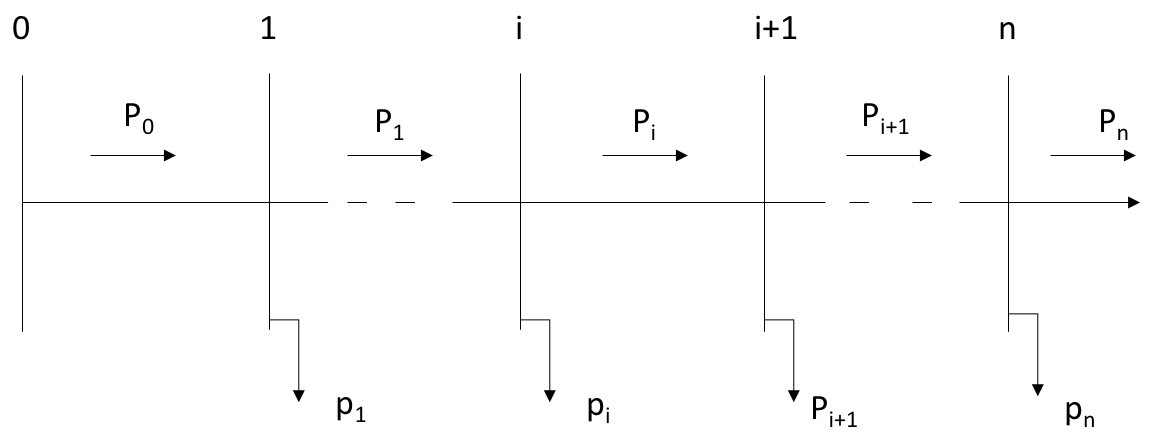
\includegraphics[scale=0.2]{pfs.png}
\caption{Diagram of a radial distribution network}
\label{pf}
\end{figure}

The DS could only import energy from the transmission system. The load in the DS is served by the DS DG as well as the TS energy import.


The goal of the DS optimization problem is to compute the DG schedule $p^d_{g,t}$ , and  energy import $p^{im}_{t}$ schedule, dispatchable load profile $l^d_{t}$, the upward/downward  DR $dr_{t}^{up}$, $dr_{t}^{dn}$ provided by the dispachable load. The lower level optimization variables are denoted by the vector $y_t$, and include:
\begin{align*}
y_t=[&p^d_{i,t}, p^{im}_{t}, dr_{i,t}^{up},dr_{i,t}^{dn},l^d_{i,t}]
\end{align*} 

The objective of the DS optimization is to minimize the DS operation cost including its DG cost,  energy import cost from the TS, and DR cost and maximize its DL utility and DR revenue.

\textbf{\emph{Objective function:} }
\begin{align*}
f(\{y_t\}^{T}_{t=1}) =& \sum_{t=1}^{T}\sum_{i=1}^{N^d_b}(C^{d1}_i p^d_{i,t} +C^{d2}_g p^d_{i,t}  p^d_{i,t} +p^{im}_{t}c^{im}_{t}\\
+ &C^{dr1} (dr^{up}_{i,t} + dr^{dn}_{i,t} ) \\
+ &C^{dr2} (dr^{up}_{i,t}dr^{up}_{i,t} + dr^{dn}_{i,t}dr^{dn}_{i,t}  ) \\
+ &C^{d}(\overline{P}^d_{i}-p^d_{i,t})(\overline{P}^d_{i}-p^d_{i,t})\\
- &p^{dr}_{t}(dr_{i,t}^{up}+dr_{i,t}^{dn}))
\end{align*}

The constraints for the DS are given below. The $\lambda$ and $\mu$ variables next to the constraints are the dual variables associated with the corresponding inequality and equality constraints.

\textbf{\emph{DG constraints:} }
\begin{align}
&\underline P^d_{i}\leq p^d_{i}\leq  \overline P^d_{i}\label{genlim}, \lambda_{1,i,t},\lambda_{2,i,t},t\in{1,...,T} ,i\in{1,...,N_b^d} 
\end{align}
Eq (\ref{genlim}) limits the generator's output within the upper and lower bound.\\

\textbf{\emph{Power flow constraints:} }
\begin{align}
& P_{i+1,t} = P_{i,t} - (L^{ie}_{i,t} + l^d_{i,t} - p^d_{i,t}) \nonumber\\
& t\in{1,...,T} ,\mu_{1,i,t},i\in{1,...,N_b^d}  \label{pfc}\\
&  \underline P_{i} \leq P_{i,t} \leq  \overline P_{i}, t\in{1,...,T}, \lambda_{3,i,t},\lambda_{4,i,t}, i\in{1,...,N_b^d}\label{pfcs}
\end{align}
Eq (\ref{pfc}) regulates the power flow between nodes in the distribution system. Eq (\ref{pfcs}) bounds the power flow within the line limits in the distribution system. Note that $P_{1,t}$ is the DS energy import $p^{im}_t$. \\

\textbf{\emph{Dispatchable load constraint:} }
\begin{align}
&\underline{L}^d_{i}\leq l^d_{i}\leq \overline{L}^d_{i,t}\label{dl}, \lambda_{5,i,t},\lambda_{6,i,t},t\in{1,...,T},i\in{1,...,N_b^d} 
\end{align} 
Eq (\ref{dl}) constrains the dispatchable loads within predefined bounds. 

\textbf{\emph{DR constraints:} }
\begin{align}
&0\leq dr_{i,t}^{up}\leq S^(dr)*l^{i,d}_t, \lambda_{7,i,t},\lambda_{8,i,t},t\in{1,...,T}, i\in{1,...,N_b^d}  \label{dlu1}\\
&0\leq dr_{i,t}^{dn}\leq S^(dr)*l^{i,d}_t, \lambda_{9,i,t},\lambda_{10,i,t},t\in{1,...,T}, i\in{1,...,N_b^d}  \label{dlu2}
\end{align} 
The amount of DR is set to be within a certain percentage defined by the DR scale factor $S^(dr)$ of the DL, which is reflected in Eq (\ref{dlu1}), (\ref{dlu2}).

%\textbf{\emph{Import and Export constraints:} }
%\begin{align}
%& 0 \leq  p^{im}_t, \lambda_{9,t}, t\in{1,...,T} \label{dlu3}
%\end{align}
%The DG import power is defined to be non-negative as shown in Eqn (\ref{dlu3}).
%
%\textbf{\emph{Power balance constraint:} }
%\begin{align}
%&p^d_{t} -L^i_{t}-l^d_{t} = -p^{im}_{t}, \mu_{2,t}, t\in{1,...,T}\label{6}
%\end{align}
%Eq (\ref{6}) ensures the power balance within the MG system.\\

Finally, the MG optimal dispatch can be formulated as: 
\begin{subequations}
\begin{align}
\text{min}_{\{y_t\}^{T}_{t=1}} & f\left(\{y_t\}^{T}_{t=1}\right)\nonumber\\
\text{s.t.  }  & (10) - (15)\nonumber
\end{align}
\end{subequations}

\subsection{Reformulation to a Single Level Problem}
If the lower level problem is convex and satisfies certain regularity conditions \cite{convex}, it can be replaced by its Karush-Kuhn-Tucker(KKT) conditions \cite{bilevel1}, the formulation in (\ref{prime}) becomes a single -level problem reformulation as follows:


\begin{align}
&\argminC_{x\in X, y\in Y}F\left(x,y\right)\nonumber\\
\text{st:  } & G_i\left(x,y\right)\leq 0, \text{for   }  i \in \{1,2,...,I\}\nonumber\\
& H_k\left(x,y\right)= 0, \text{for   }  k \in \{1,2,...,K\}\nonumber\\
&g_i\left(x,y\right)\leq 0, \text{for   }  j \in \{1,2,...,J\}\nonumber\\
&h_m\left(x,y\right)\leq 0, \text{for   }  m \in \{1,2,...,M\}\nonumber\\
&\text{dual feasibility: }\lambda_i\geq 0, \text{for   }  i \in \{1,2,...,I\}\nonumber\\
&\text{complementary slackness: }\nonumber \\
&\lambda_i*g_i\left(x,y\right)= 0, \text{for   }  i \in \{1,2,...,I\}\nonumber\\ 
&\text{stationarity: }\nabla \textit{L}(x,y,\lambda,\mu)=0\nonumber\\ 
& where:\nonumber\\ 
 &  \textit{L}(x,y,\lambda)=f(x,y)+\sum_{i=1}^{J}\lambda _ig_i(x,y)+\sum_{m=1}^{M}\mu _mh_m(x,y)\nonumber
\end{align}


The lower level problem in this study is a convex optimization problem and satisfies Slater's condition, which is one of the sufficient conditions for strong duality theorem \cite{convex}. Therefore, the lower level problem could be replaced by its KKT conditions. The KKT conditions are given below:\\

\textbf{\emph{Stationarity}}: \\
For stationarity, the derivative of the lagrangian function  $\textit{L}(x,y,\lambda)$ is taken with respect to each optimization variable. For example, eq(\ref{lam1}) is the derivative of the lagrangian function with respect to $p^d_{i,t}$.
\begin{align}
& 2*C^{d2}_i*p^d_{i,t} + C^{d1}_i + \lambda_{2,i,t}-\lambda_{1,i,t}+\mu_{1,i,t} =0 \nonumber\\ 
& t\in{1,...,T},i \in \{1,...,N^d_b\} \label{lam1}\\
& 2*C^{dr2}_i*dr^{up}_{i,t} + C^{dr1}_i - p ^{dr}_t + \lambda_{8,i,t}-\lambda_{7,i,t} =0 \nonumber\\ 
& t\in{1,...,T},i \in \{1,...,N^d_b\}  \\
& 2*C^{dr2}_i*dr^{up}_{i,t} + C^{dr1}_i - p ^{dr}_t + \lambda_{8,i,t}-\lambda_{7,i,t} =0 \nonumber\\ 
& t\in{1,...,T},i \in \{1,...,N^d_b\} \\
& p^{im}_t -\mu_{1,1,t}+ \lambda_{4,1,t}-\lambda_{3,1,t} =0, t\in{1,...,T}, i=1 \\
& \mu_{1,i-1,t} -\mu_{1,i,t}+ \lambda_{4,i,t}-\lambda_{3,i,t} =0,  \nonumber\\ 
& t\in{1,...,T},i \in \{2,...,N^d_b\} \\
%& \mu_{1,i-1,t} -\mu_{1,i,t}+ \lambda_{4,i,t}-\lambda_{3,i,t} =0, t\in{1,...,T} \\
& 2*C^{d}*l^d_{1,t} + C^{d}*\overline{L}^d_{i,t} + \lambda_{6,1,t}-\lambda_{5,1,t}\nonumber\\
&-\lambda_{8,1,t}-\lambda_{10,1,t} =0 , t\in{1,...,T}, i = 1  \label{lam1}\\
& 2*C^{d}*l^d_{i,t} + C^{d}*\overline{L}^d_{i,t} + \lambda_{6,i,t}-\lambda_{5,i,t}\nonumber\\
& -\lambda_{8,i,t}-\lambda_{10,i,t}+\mu_{1,i,t}=0 , t\in{1,...,T}, i\in{2,...,N^d_b}  \label{lam1}
\end{align}

 \textbf{\emph{Dual feasibility}}: \\
For dual feasibility, all dual variables need to be non-negative.
\begin{align}
\lambda_{1,t} ... \lambda_{10,t} , t\in{1,...,T} \geq 0 
\end{align}
\textbf{\emph{Complementary slackness}}: \\
For complementary slackness, the product of the dual variables and their corresponding inequalities need to be zero.
\begin{align}
& \lambda_{1,i,t}*(p^d_{i,t}-\underline P^d_i) = 0, t\in{1,...,T}, i\in{1,...,N^d_b}  \\
& \lambda_{2,i,t} *(p^d_{i,t}-\overline P^d_i) = 0 , t\in{1,...,T}, i\in{1,...,N^d_b}  \\
& \lambda_{3,i,t}*(P_{i,t}-\overline P_i) = 0 , t\in{1,...,T}, i\in{1,...,N^d_b}  \\
& \lambda_{4,i,t}*(P_{i,t}-\underline P_i) = 0 , t\in{1,...,T}, i\in{1,...,N^d_b}  \\
& \lambda_{5,i,t}*(l^d_{i,t}-\overline L^d_{t}) = 0 , t\in{1,...,T} , i\in{1,...,N^d_b} \\
& \lambda_{6,i,t}*(l^d_{i,t}-\underline L^d_t) = 0 , t\in{1,...,T}, i\in{1,...,N^d_b}  \\
& \lambda_{7,i,t}*dr_{i,t}^{up} = 0 , t\in{1,...,T} , i\in{1,...,N^d_b} \\
& \lambda_{8,i,t}*(dr_{i,t}^{up}-0.2*l^d_{i,t}) = 0 , t\in{1,...,T} , i\in{1,...,N^d_b} \\
& \lambda_{9,i,t}*dr_{i,t}^{dn} = 0, t\in{1,...,T} , i\in{1,...,N^d_b}  \\
& \lambda_{10,i,t}*(dr_{i,t}^{dn}-0.2*l^d_{i,t}) = 0 , t\in{1,...,T} , i\in{1,...,N^d_b} 
\end{align}

This reformulation is not easy to solve mainly due to the non-convexity in the complementary slackness and bilinear terms in the objective function. The big-M reformulation is used to transform the complementary conditions to mixed integer constraints. The technical details of the Big-M method is given in the appendix. 

According to strong duality theorem, the optimal objective function value of the lower level optimization dual problem equals the optimal objective function value of the lower level optimization primal problem.  As a result, the bilinear terms $-p^{im}_{t}c^{im}_{t}+p^{dr}_{t}(dr_{t}^{up}+dr_{t}^{dn})$ in the lower level objective function, which also appear in the upper level objective function, could be expressed as linear terms using the objective function of the dual problem. The lower level dual problem objective function is as follow:\\
\begin{equation*}
\begin{array}{lcl}
D(\{\lambda_t,\mu_t\}^{T}_{t=1}) &=& \sum_{t=1}^{T}\sum_{i=1}^{N^d_b}(-C^{d2}p^{d}_{i,t}p^{d}_{i,t} - C^{ld}l^{d}_{i,t}l^{d}_{i,t} \\
&-& l^{d}_{i,t}\mu_{i,t} + \lambda_{3,i,t} \underline{P}_{i,t} -\lambda_{4,i,t} \overline{P}_{i,t} \\
&+&\lambda_{5,i,t} \overline{L}^{d}_{i,t} -\lambda_{6,i,t} \underline{L}^{d}_{i,t}\\
&+&\lambda_{1,i,t} \overline{P}^{d}_{i} -\lambda_{2,i,t} \underline{P}^{d}_{i})
\end{array}
\label{eqn:obj}
\end{equation*}

The bilinear terms $-p^{im}_{t}c^{im}_{t}+p^{dr}_{t}(dr_{t}^{up}+dr_{t}^{dn})$ in the upper level objective function are represented as:
\begin{align*}
y = & \sum_{t=1}^{T}\sum_{i=1}^{N^d_b}(C^{d1}_i p^d_{i,t} +C^{d2}_g p^d_{i,t}  p^d_{i,t} \\
+ &C^{dr1} (dr^{up}_{i,t} + dr^{dn}_{i,t} ) \\
+ &C^{dr2} (dr^{up}_{i,t}dr^{up}_{i,t} + dr^{dn}_{i,t}dr^{dn}_{i,t}  ) \\
+ &C^{d}(\overline{P}^d_{i}-p^d_{i,t})(\overline{P}^d_{i}-p^d_{i,t})) - D(\{\lambda_{i,t},\mu_{i,t}\}^{T,N^d_b}_{t=1,i=1}) 
\end{align*}

%\begin{align*}
%\sum_{t=1}^{T}(C^{m1}_g p^m_{g,t} +C^{m2}_g p^m_{g,t}  p^m_{g,t} +C^bb_t + C^{dr1} dr^{up}_{g,t} + dr^{dn}_{g,t}  +\\
%+C^{dr2} (dr^{up}_{g,t}dr^{up}_{g,t} + dr^{dn}_{g,t}dr^{dn}_{g,t}  ) - C^d_{t}l^d_{t}) - D(\{\lambda_{i,t},\mu_{i,t}\}^{T,N^d_b}_{t=1,i=1}) 
%\end{align*}

The reformulated upper level objective function is as follow:\\
\begin{equation*}
\begin{array}{lcl}
F\left(\{x_t,y_t, \lambda_{t,i}, \mu_{t,i}\}^{T,N^d_b}_{t=1,i=1}\right) &=& \sum_{t=1}^{T}\sum_{g=1}^{G}(C^c_{g,t} w_{g,t}+C_{g,t} p_{g,t} \\
&+&C^r_{g}(r_{g,t}^{up}+r_{g,t}^{dn}) - y
\end{array}
\label{eqn:obj}
\end{equation*}

The reformulated single level problem has the following format:\\
\begin{subequations}
\begin{align}
\text{min}_{\{x_t,y_t, \lambda_t, \mu_t\}^{T}_{t=1}} & F\left(\{x_t,y_t, \lambda_t, \mu_t\}^{T}_{t=1}\right)\nonumber\\
\text{st:   } & (2)-(34)\nonumber
\end{align}
\end{subequations}

With the big-M reformulation, a set of binary variables and additional constants are introduced. The bilevel problem becomes a single level mixed integer linear problem and could thus be solved with a wide range of commercial solvers such as Cplex and Gurobi. 


%\subsection{Optimization Model}
%\subsection{Representing Wind Uncertainty}
%\input{windsec}
\section{Numerical Results}\label{sec:Results}
%!TEX root = HICSS51.tex
In this section, the transmission model described in Section~\ref{sec:Model} is applied to the IEEE 30-bus system, shown in Fig.
\ref{fig:wee}. Interested readers are referred to \cite{zimmerman2009matpower} for
detailed parameters of the TS. The parameters of the 15 MW DS with 50\% DL and a DR scale factor of 30\% is listed in the appendix.  A wind farm is positioned at bus 8 in the TS to provide renewable generation. A DS is also connected at bus 8 to provide DR to offset the renewable forecast errors.
\begin{figure}[H]
\centering
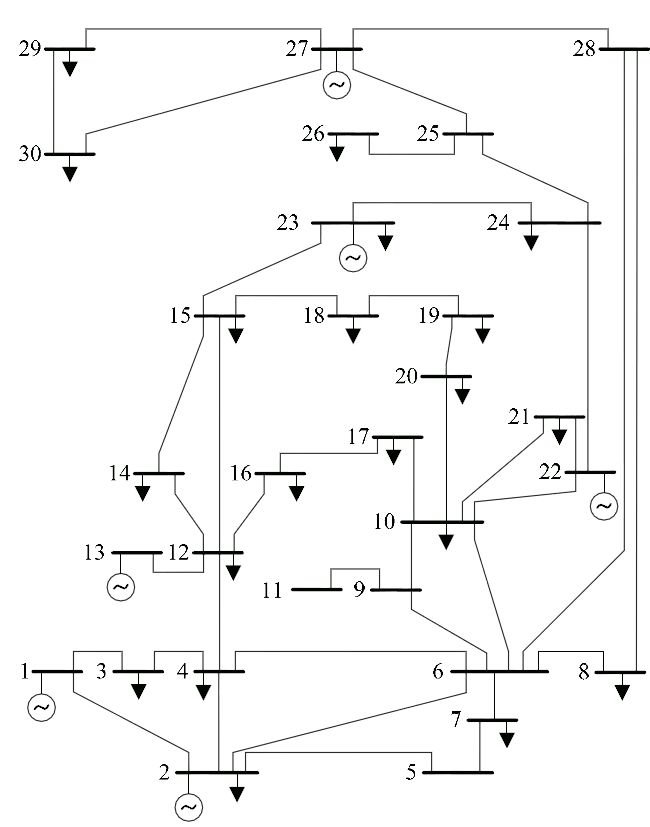
\includegraphics[scale=0.4]{IEEE_30bus.png}
\caption{IEEE 30 Bus System}
\label{fig:wee}
\end{figure}

The wind data for the wind farms in the TS are selected from the
NREL-Eastern Wind Integration Study dataset \cite{energy2010eastern}.
Using three years of data, 24-hour trajectories are grouped
to identify a set of 54 similar trajectories, with a common initial
condition. The set of trajectories was used
to represent the realizations of a similar forecast. The central
trajectory of the group was selected as the wind forecast,
and the remaining were used to estimate the distribution of
forecast errors, as described in \cite{anderson2011wind}. From the forecast error
distribution, 10000 scenarios are used to generate a robust
wind error scenario set. 

%For the MG import price, the locational marginal price for each buse in the TS without the MG is precomputed for a wide range of loading conditions. Then a first order equation is fitted between the price and the import quantity. This way the import price is approximated as a linear function of the import quantity as below:
%\begin{subequations}
%\begin{align}
%C^{im}_t = a*P^{im}_t + b
%\end{align}
%\end{subequations}                                                            
%where $a$ and $b$ are two constants representing the slope and intercept of the pricing equation. The method enables a dynamic pricing scheme which accounts for varying system loading conditions and at the same time preserves the convexity of the problem. The export price is defined as 90\% of the import price at each quantity to avoid the market flaw of buying energy and selling back to make money. This pricing scheme might not be the best pricing scheme. The optimal pricing scheme is out of the focus and scope of the work.

The objective of this work is to analyze different factors that affect the WP in the TS and the operational cost of the two systems in this co-optimization framework as well as the standalone framework.

The definition of WP is based on the wind power capacity penetration defined by the European Wind Energy Association \cite{european2012wind}. It is the ratio of the installed wind capacity divided by the peak system load.


\subsubsection{Base Case: no DR}
For benchmarking purpose, a base case study is carried out first. The DL level is 50\%. The DR function in the DS is disabled. The results are given in Table \ref{transbus}.

%The To generate some benchmarks, a wind farm is positioned at different buses in the TS with no MG. The maximum WP in each case is recorded.

\begin{table}[H]
\centering
\begin{tabular}{ |c|c|c| } 
 \hline
 Max WP & TS Cost & DS Cost \\ 
 \hline
29\% & 8798 & 1697 \\ 
 \hline
\end{tabular}
\caption{ Base Case Results}
 \label{transbus}
\end{table}

\subsubsection{Case 1: different DL levels with DR}
In this case, the DR function of the DS is enabled and maintained at a level of 30\%. The WP and costs of the two systems at different DL levels are recorded in Table \ref{transbuse}.

\begin{table}[H]
\centering
\begin{tabular}{ |c|c|c|c| } 
 \hline
DL Level& Max WP & TS Cost & DS Cost \\ 
 \hline
25\% & 30\% & 8568 & 2720 \\ 
 \hline
50\% & 31\% & 8771 & 1660 \\ 
 \hline
75\% & 33\% & 9110 & 180 \\ 
 \hline
\end{tabular}
\caption{Results at Different DL Levels}
 \label{transbuse}
\end{table}

From Table \ref{transbuse}, the WP increases with an increasing DL level, however the increase in WP is not significant. That is because the DS size is relatively very small and the amount of DR it could provide is very limited. Looking at the system costs, the TS cost increases due to the increased requirement for reserves to compensate for the increased wind uncertainty. The DS cost decreases significantly with the increased DL level as it has more DR capacity with more DL to make more revenue. In addition, the flexibility with more DL could enable more load curtailing at expensive period ,which also reduces the system cost. Compared to the base case, the DR generates considerable cost savings for both systems as the base TS case cost at 29\% WP is even greater than the 31\% WP in this case. Moreover, the DR also reduces the DS cost for the same setting compared to the base case.

\subsubsection{Case 2: different DR levels}
In this case, the DR function of the DS is enabled and varied at different levels. The DL level is maintained at 50\%. The WP and costs of the two systems at different DL levels are recorded in Table \ref{transbusf}.

\begin{table}[H]
\centering
\begin{tabular}{ |c|c|c|c| } 
 \hline
DR Level & Max WP & TS Cost & DS Cost \\ 
 \hline
15\% & 30\% & 8795 & 1706 \\ 
 \hline
30\% & 31\% & 8821 & 1660 \\ 
 \hline
45\% & 33\% & 8862 & 1644 \\ 
 \hline
\end{tabular}
\caption{Results at Different DL Levels}
 \label{transbusf}
\end{table}

From Table \ref{transbusf}, the WP increases with an increasing DR level, once again the increase in WP is not significant. The reason is the same as before. Looking at the system costs, the TS cost increases due to the increased requirement for reserves to compensate for the increased wind uncertainty. One interesting thing to note is that the increase in TS cost in this case is smaller than the previous case. That is because in the previous case the amount of DR does not necessarily increase for all periods with an increased amount of DL as the DL setpoint could be very low for some periods and thus have very limited DR for those periods, so those periods still incur high cost increase with a higher WP. In the contrary, an increasing DR level at a constant DL guarantees more DR in this case and could more effectively reduce the cost increase in the TS with more wind uncertainty. The DS cost decreases with an increasing DR level but not as significantly as the previous level. That is due to the fact that the DS in the previous case saves money not only from DR but also from load curtailing. 

%\begin{table}[H]
%\centering
%\begin{tabular}{ |c|c|c| } 
% \hline
% Wind Bus & Max WP & Reason \\ 
% \hline
%5 & 38\% & Use up generator reserve \\ 
% \hline
%8 & 28\% & Reach transmission limit\\ 
% \hline
%15 & 38\% & Use up generator reserve \\ 
% \hline
%30 & 28\% & Reach transmission limit \\ 
% \hline
%8 and 30 & 38\% & Use up generator reserve \\ 
% \hline
%\end{tabular}
%\caption{ WP at different buses}
% \label{transbus}
%\end{table}

%As the TS has a network with limits on transmission lines, different buses have different capacities in terms of renewable injection. Table \ref{transbus} shows that bus 8 and 30 allows smaller WPs compared to bus 5 and 15 as bus 8 and 30 are connected to transmission lines with smaller capacity. For bus 5 and 15, the connected line capacity is large enough to use up the generator reserve to achieve maximum WP. When there are two wind farms at bus 8 and 30, all the generator reserve is used to account for the wind forecast deviation as the combined line capacity at those two buses is large enough to use up the generator reserve. Therefore, wind farms should avoid buses with tight transmission constraints in terms of their placement. The method to find buses that are more prone to violate transmission constraints in given in \cite{liu2016quantifying}. As a result, wind farms should be placed at buses with generous transmission capacity and possibly at multiple locations to achieve high level of WP.
%
%\subsubsection{WP with a MG}
%To illustrate the effects of MG on the WP, a 25MW MG with 50\% DL is connected to the wind buses in the previous section. Here the DL percentage is defined as the ratio of the maximum DL and the sum of maximum DL and non-DL. The size of the MG (25MW in this case) is defined as the generation capacity of the MG. The WP with and without the MG is given in Fig.\ref{fig:wp}.
%
%%\begin{figure}[H]
%%\centering
%%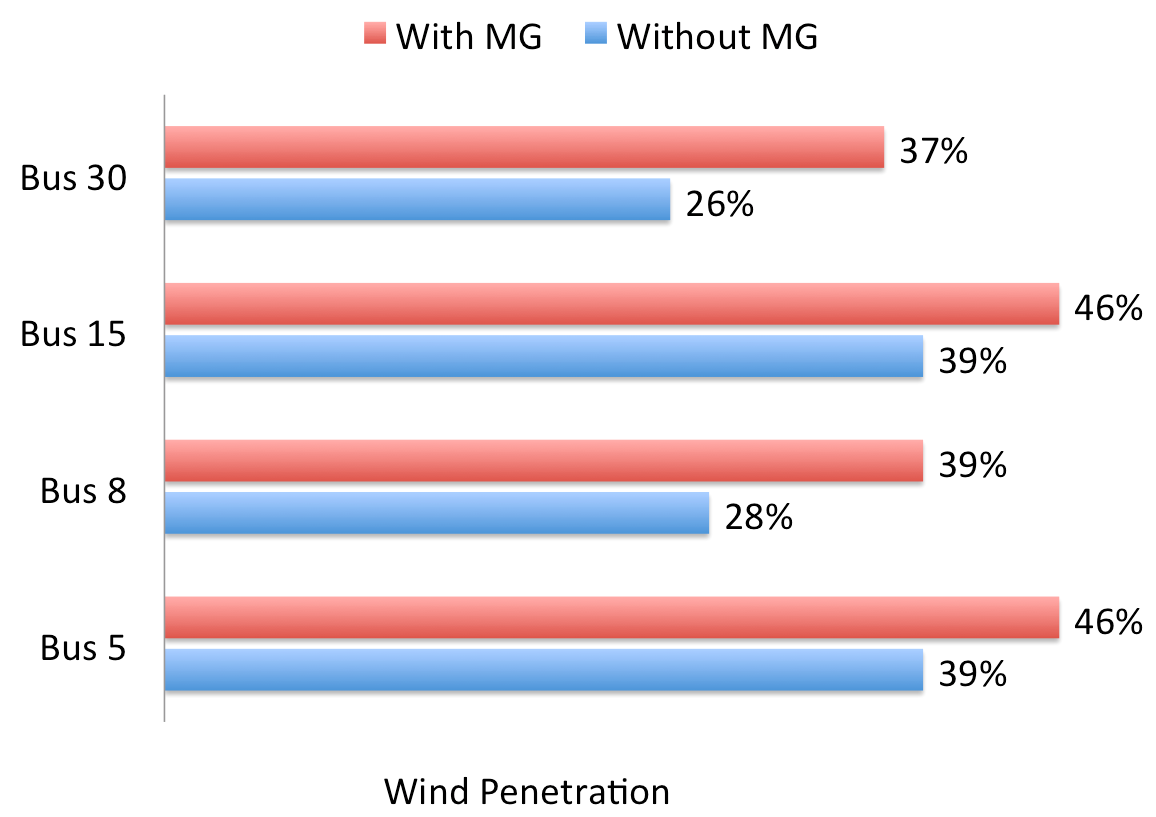
\includegraphics[scale=0.25]{windp.png}
%%\caption{WP with and without MG at different buses}
%%\label{fig:wp}
%%\end{figure}
%
%Fig.\ref{fig:wp} illustrates that the WP in general increases since the DR provided by the MG could act as reserve and locally offset some wind forecast error at the wind bus. The penetration increase for bus 8 and 30 is more than that of bus 5 and 15 as the MG and TS energy exchange at bus 8 and 30 frees some line capacity for the generator reserves. This case shows that the MG could alleviate congestion under the current energy exchange pricing scheme. This observation is consistent with the results in \cite{liu2016quantifying}. Therefore, for congestion management purpose, MGs should be placed at buses with congestions under this optimization framework.
%% and the wind injection consumes some line capacity. 
%% Due to power flow constraints, some simulation results show that MG might not always result in an increase in WP as the net injection into the bus could cause congestion and decrease the supply of generator reserve. For example, when the MG and wind farm are both at bus 8 and the MG energy cost is very low for some periods, the MG will export energy into the TS and cause serious congestion, the WP in this case could be equal or even below 28\%. A key lesson from this counter example is that the MG makes decision to maximize its own welfare which might not help with maximizing WP. 
%Table \ref{transbuss} shows the the maximum WP when the MG is placed at different buses from the wind farm bus. This table shows that when the MG and wind farm are at different buses, the  WP level could only be less than that when they are at the same bus as the later case could bypass transmission constraints and directly offset wind forecast error, which is not possible for the former case. 
%
%\begin{table}[H]
%\centering
%\begin{tabular}{ |c|c|c| } 
% \hline
% Wind Bus & MG Bus & Max WP \\ 
% \hline
%5 & 8 & 45\% \\ 
% \hline
%5 & 15 & 45\% \\ 
% \hline
%5 & 30 & 45\% \\ 
% \hline
%8 & 5 & 28\%\\ 
% \hline
%8 & 15 & 28\% \\ 
% \hline
%8 & 30 & 28\% \\ 
% \hline
%\end{tabular}
%\caption{ WP with the wind farm and MG at different buses}
% \label{transbuss}
%\end{table}


%In order to truly achieve the maximum WP that both systems could support, a more sophisticated pricing schemes need to be designed that links the WP to MG's wellfare. However, this is out

%Two typical scenarios that do not result in WP increase is illustrated in Table \ref{noinc}.

%\begin{table}[h]
%\centering
%\begin{tabular}{ |c|c|c| } 
% \hline
% Wind and MG Bus & Scenario & Max WP \\ 
% \hline
%8 & 27\% & Violate transmission limit due to too much energy export from MG  \\ 
% \hline
%30 & 28\% & Violate transmission limit due to too much downward DR \\ 
% \hline
%\end{tabular}
%\caption{ WP at different buses}
% \label{transbus}
%\end{table}

%\subsubsection{WP for different MG sizes and DL levels}
%As the amount of reserve is proportional to the size of the MG and the amount of DL in the MG, the WP with regards to those two factors are analyzed here. To simulate a MG with varying sizes, the MG parameters except for the ones related to the costs are scaled by the same constant. The wind farm and MG are both located at bus 5 to guarantee enough line capacity and no interference from line constraints. Fig. \ref{wpd} shows WPs for different sizes of a MG with 50\% of the loads being dispachable. Fig. \ref{wpdd} shows WPs for a 25MW MG with different levels of DLs. It can be seen from the two figures that WPs are linearly proportional to MG size and DL levels as there is more MG DR to offset the wind forecast error. 
%However, it is still possible for the MG to cause congestion anomalies at some buses as described in the previous subsection and violate the general rules here.

%\begin{figure}[H]
%\centering
%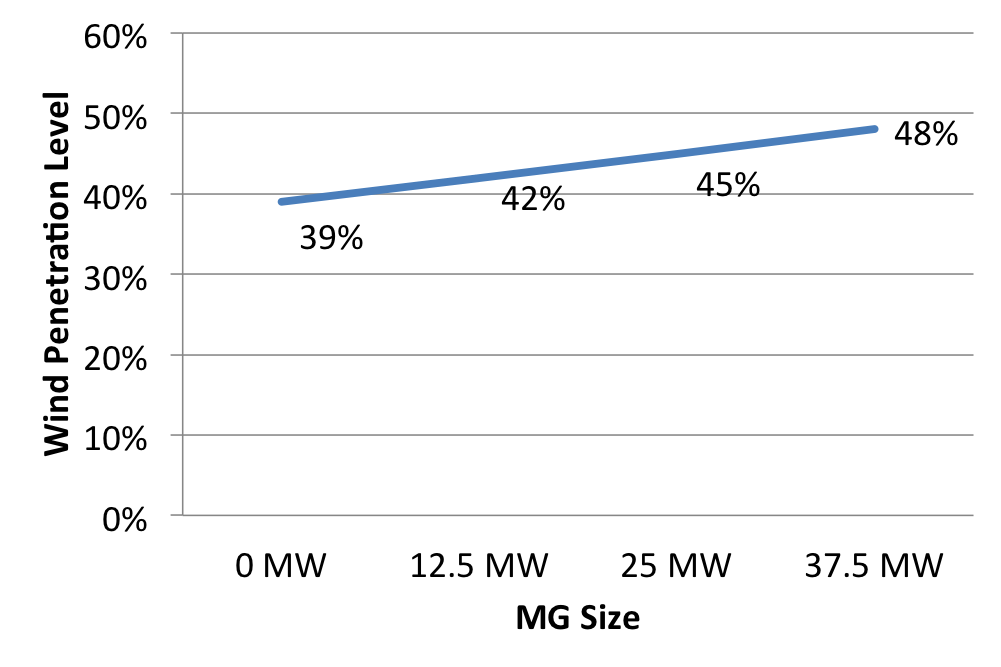
\includegraphics[scale=0.55]{windpd.png}
%\caption{WP for different MG sizes}
%\label{wpd}
%\end{figure}
%
%\begin{figure}[H]
%\centering
%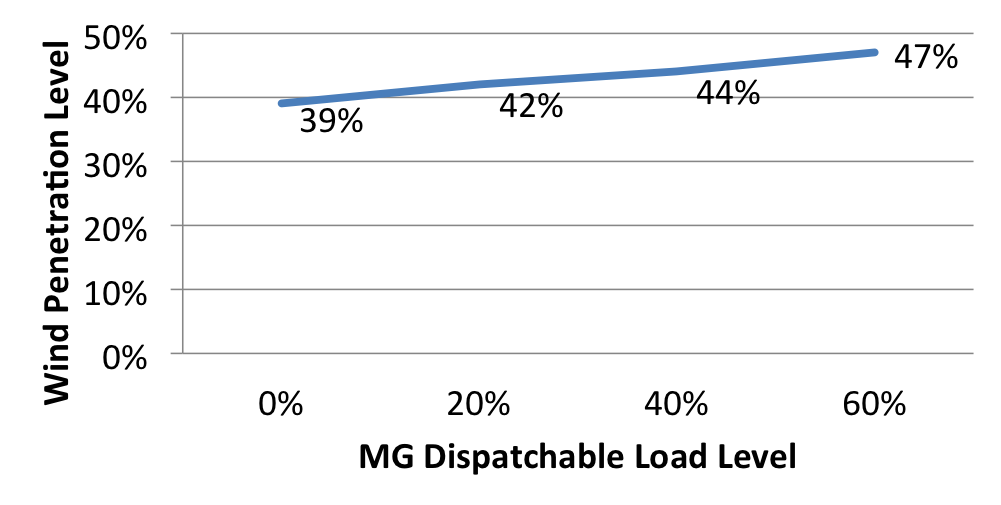
\includegraphics[scale=0.55]{windpdd.png}
%\caption{WP for different DL levels}
%\label{wpdd}
%\end{figure}

%\subsection{System Cost Results}
%One goal of the TS and MG co-optimization is to reduce the individual system's operation cost. Different factors that affect the cost of the two systems are explored in this section. For the figures in this subsection, SA stands for standalone mode, while COOP stands for co-optimization mode. In the COOP mode, the MG is able to provide DR as reserve to account for the wind forecast error in the TS and exchange energy with the TS. In the SA mode, the MG is separated from the TS and thus could not exchange energy with the TS or provide any DR.
%
%\subsubsection{WP on transmission and MG cost}
%As WP is a key concern of the future grid and also a focus of this study, the WP is varied to see the impact on the TS and MG cost. The wind farm and a 25MW MG with 50\% DL is connected to bus 5. The results are displayed in Fig. \ref{pdsize1}.

%\begin{table}[h]
%\centering
%\begin{tabular}{ |c|c|c| } 
% \hline
% WP & Transmission Cost & MG Cost \\ 
% \hline
%0\% & 9068 & 1440  \\ 
% \hline
%5\% & 9095 & 1332 \\ 
% \hline
%10\% & 9376 & 1347 \\ 
% \hline
%15\% & 9682 & 1336 \\ 
% \hline
%\end{tabular}
%\caption{ WP at different buses}
% \label{wdlevel}
%\end{table}

%\begin{figure}[H]
%\centering
%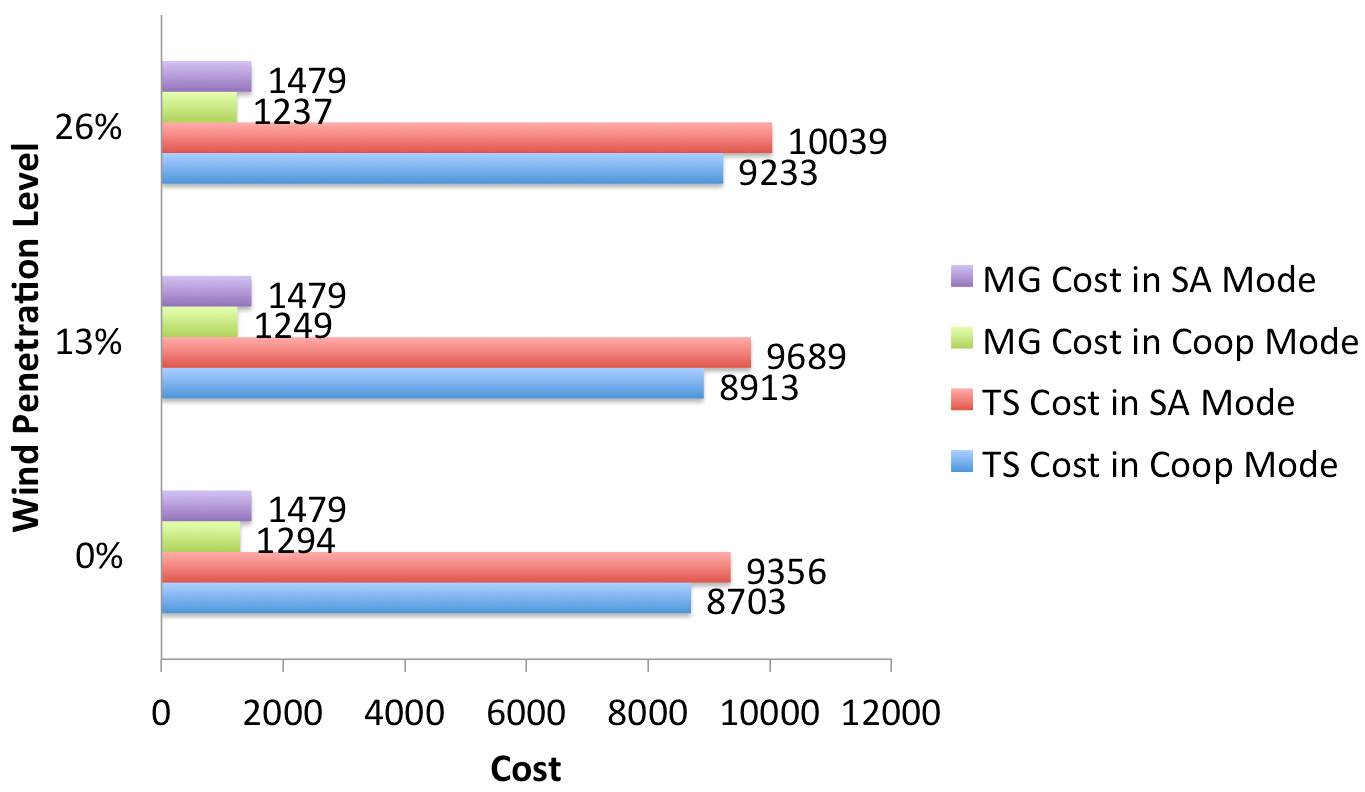
\includegraphics[scale=0.25]{wp1.png}
%\caption{TS cost for different WP levels}
%\label{pdsize1}
%\end{figure}
%
%\begin{figure}[H]
%\centering
%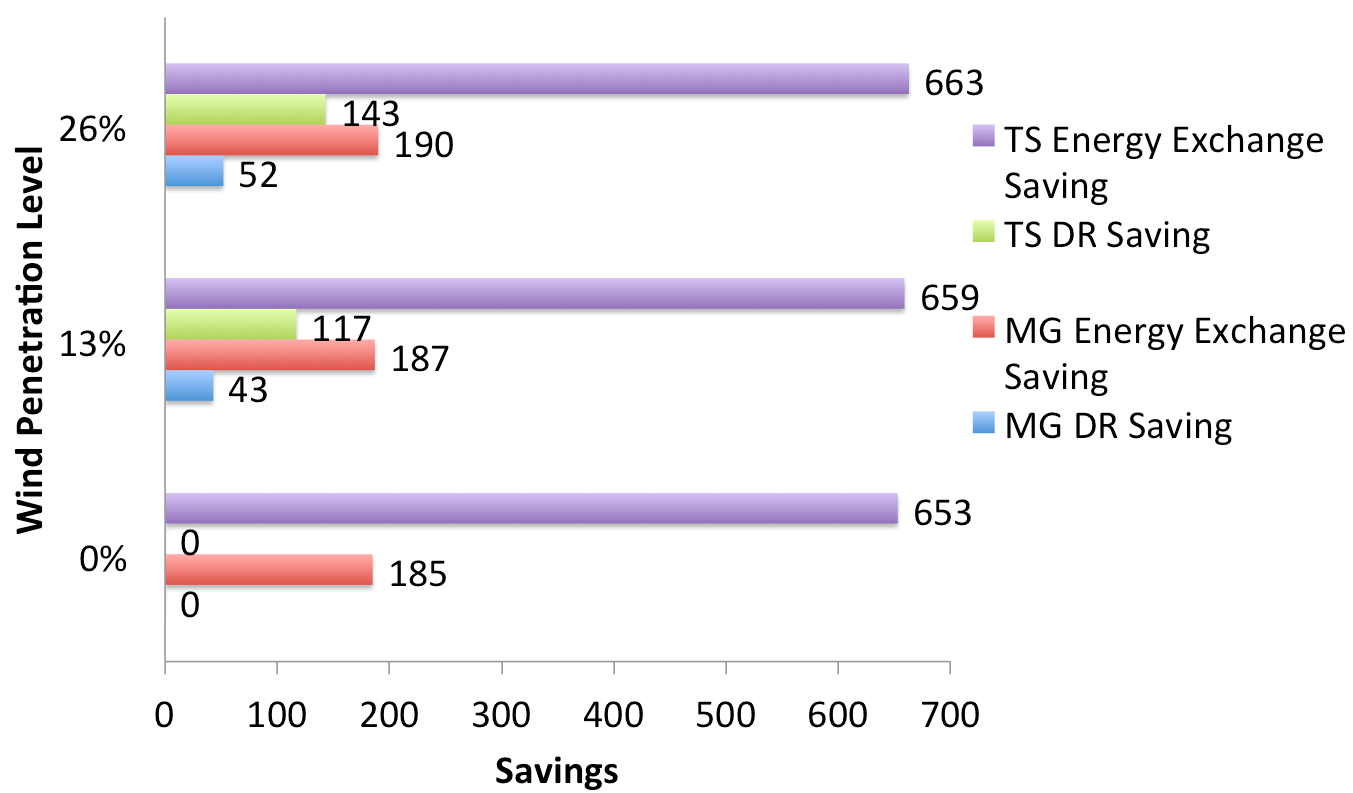
\includegraphics[scale=0.25]{wp2.png}
%\caption{TS and MG savings breakdown for different WP levels}
%\label{pdsize2}
%\end{figure}

%From Fig. \ref{pdsize1},  the operational costs of the two systems are smaller in the Coop mode due to the mutual benefits from the energy exchange and DR.   In the SA mode, the MG cost is the same for all three cases as the MG configuration stays the same for all of them. Fig. \ref{pdsize1} shows the break down of the MG and TS savings in terms of DR and energy exchange. When there is no wind, the difference in the operational cost between the operational modes is totally from the energy exchange benefits. As wind penetration increases, the DR savings for the MG and TS increase as more cheaper MG DR is engaged in the ancillary market. The energy exchange saving for the two systems are more or less the same for the three cases as the energy exchange price and quantity (mainly MG import) do not change much. This case study shows that the total saving in the Coop mode with a higher WP is greater for both systems.
%
%\subsubsection{MG size on transmission cost}
%The TS is optimized with different sizes of MG connected to bus 5 and the operation cost is reported in Fig. \ref{mgsize}.  For all the cases, the DL level in the MG is 50\%. The wind farm is connected to bus 8, and a fixed 10\% WP is used. 
%
%%\begin{figure}[H]
%%\centering
%%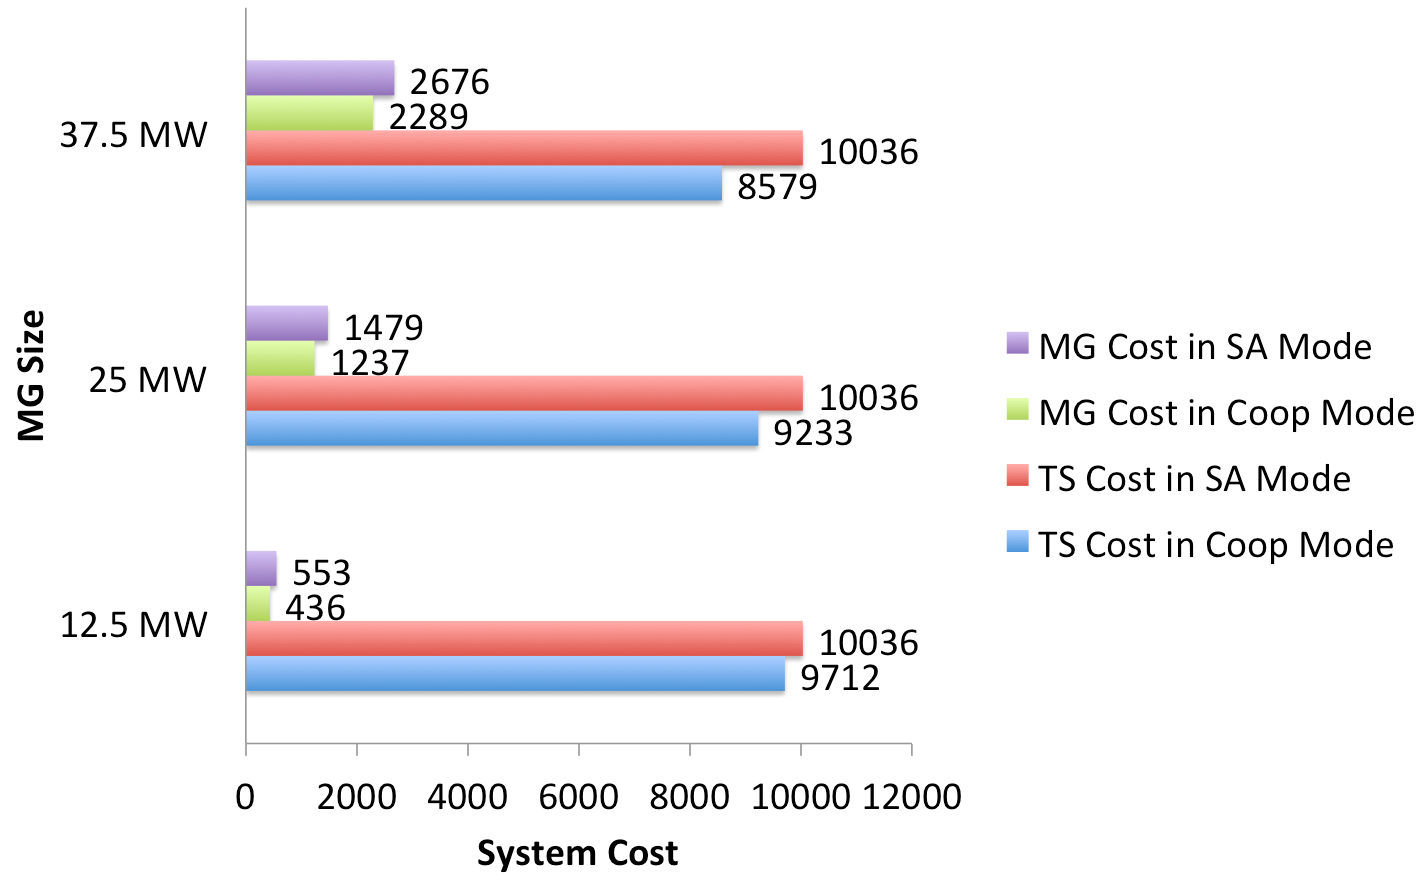
\includegraphics[scale=0.25]{mgsize1.png}
%%\caption{TS cost for different MG sizes}
%%\label{mgsize}
%%\end{figure}
%%
%%\begin{figure}[H]
%%\centering
%%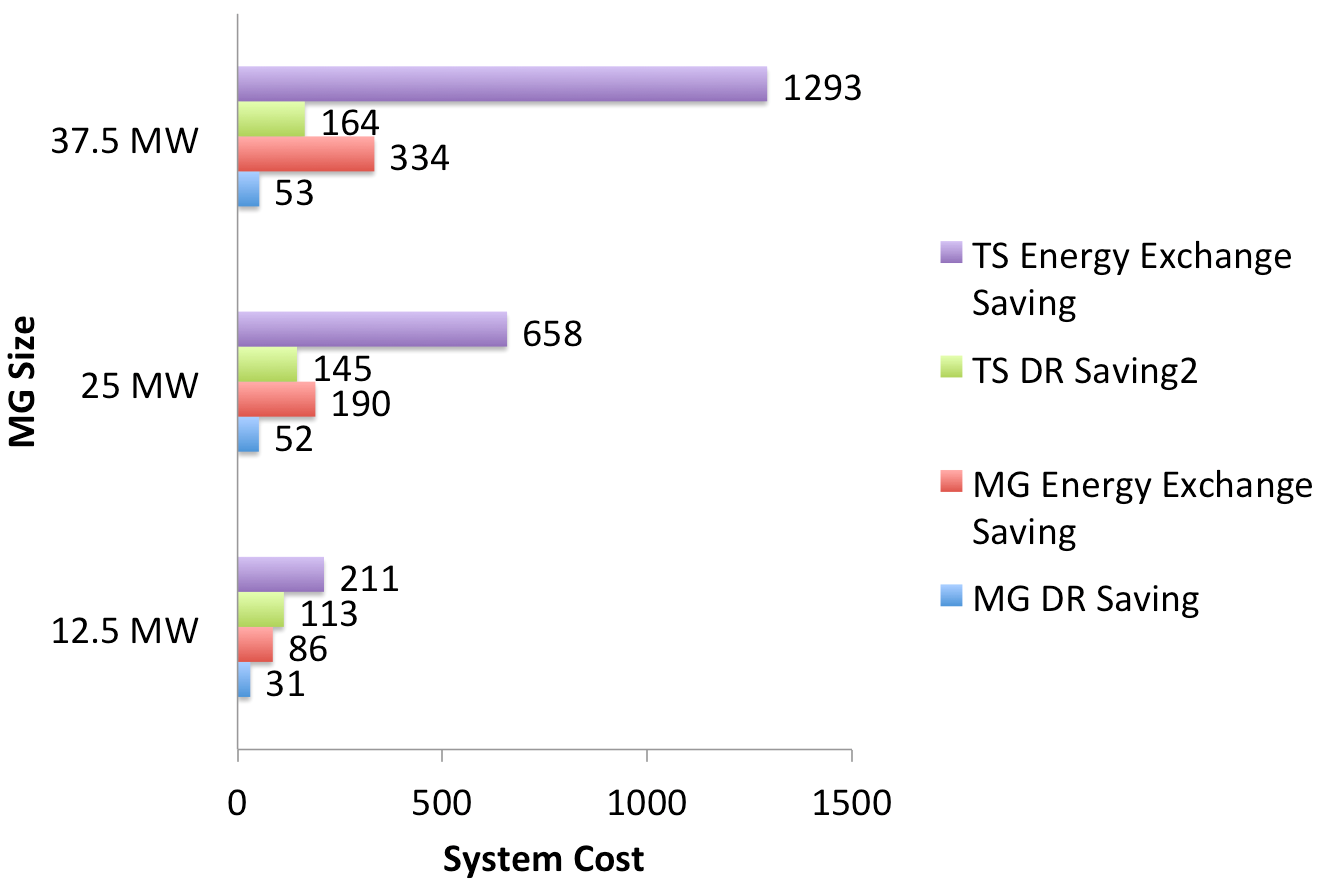
\includegraphics[scale=0.25]{mgsize2.png}
%%\caption{TS and MG savings breakdown for different MG sizes}
%%\label{mgsize2}
%%\end{figure}
%
%From Fig. \ref{mgsize}, it can be seen that in the Co-op mode the cost of the TS decreases with the increase in MG size. That is due to the increased volume of the DR and energy exchange with a larger MG. In addition, the individual system's cost is always smaller in the co-optimization mode compared to the standalone mode as both systems have opportunities to arbitrage in the energy exchange transactions in addition to the benefits from the reserve provision. In the SA mode, the TS cost is the same for all three cases as the TS configuration stays the same for all of them. Fig. \ref{mgsize2} shows the break down of the MG and TS savings in terms of DR and energy exchange. As the MG size increases, the benefits from the energy exchange for both systems increase since the energy exchange volume increases with a larger MG. The DR benefits for both systems also increase as a larger MG could provide more DR service. However the MG DR benefit does not increase much from a 25MW to a 37.5MW MG. That is because the DR price in the latter case is actually lower although the DR provision is greater. This case study shows that the total saving in the Coop mode with a bigger MG is greater for both systems.
%
%\subsubsection{MG DL level on transmission and MG cost}
%For the setting of a 25MW MG  and 10\% WP at bus 5 in the TS, the TS and MG operation cost at different levels of MG DL are reported in Fig. \ref{pdsize}.
%
%%\begin{figure}[H]
%%\centering
%%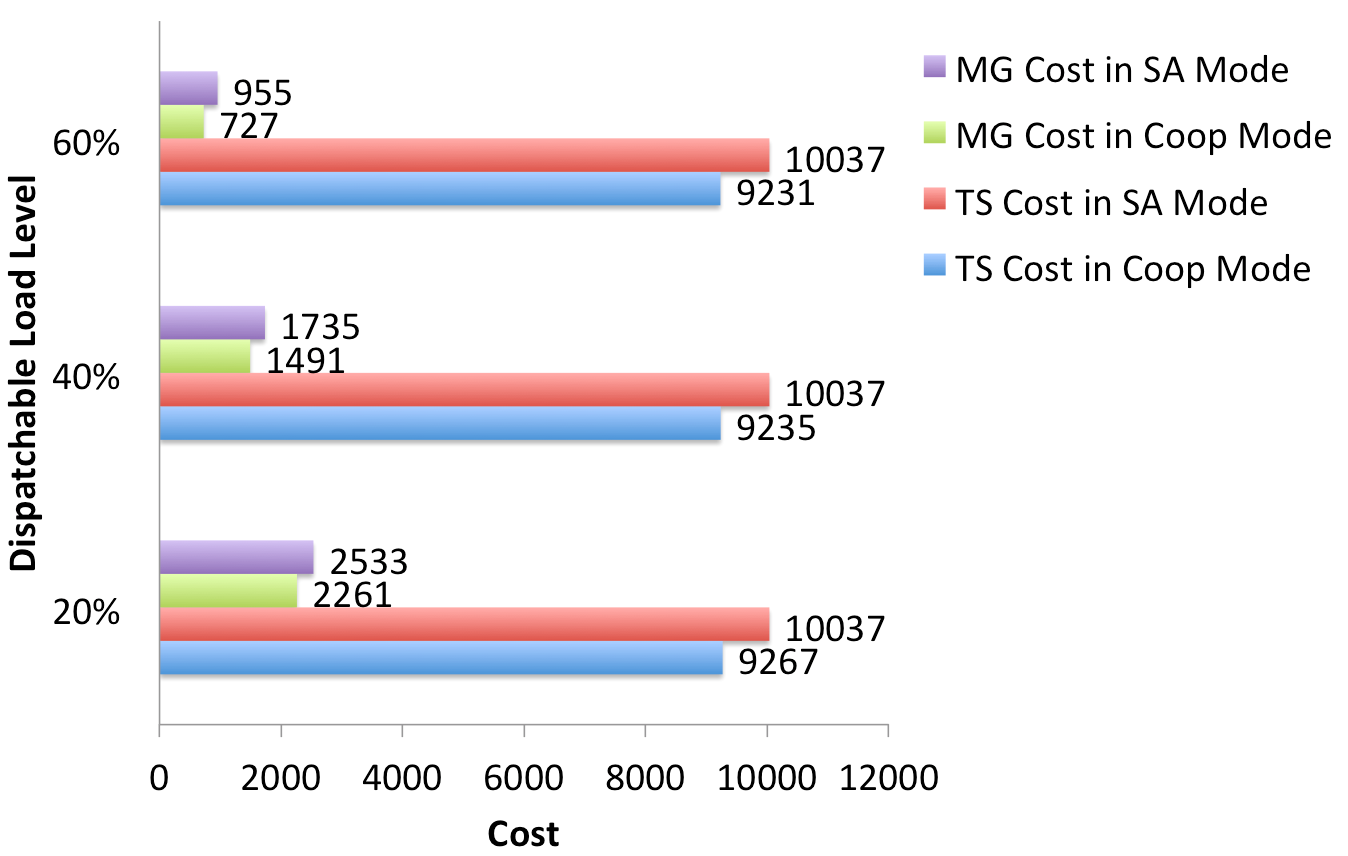
\includegraphics[scale=0.25]{pdsize1.png}
%%\caption{TS cost for different MG DL levels}
%%\label{pdsize}
%%\end{figure}
%%
%%\begin{figure}[H]
%%\centering
%%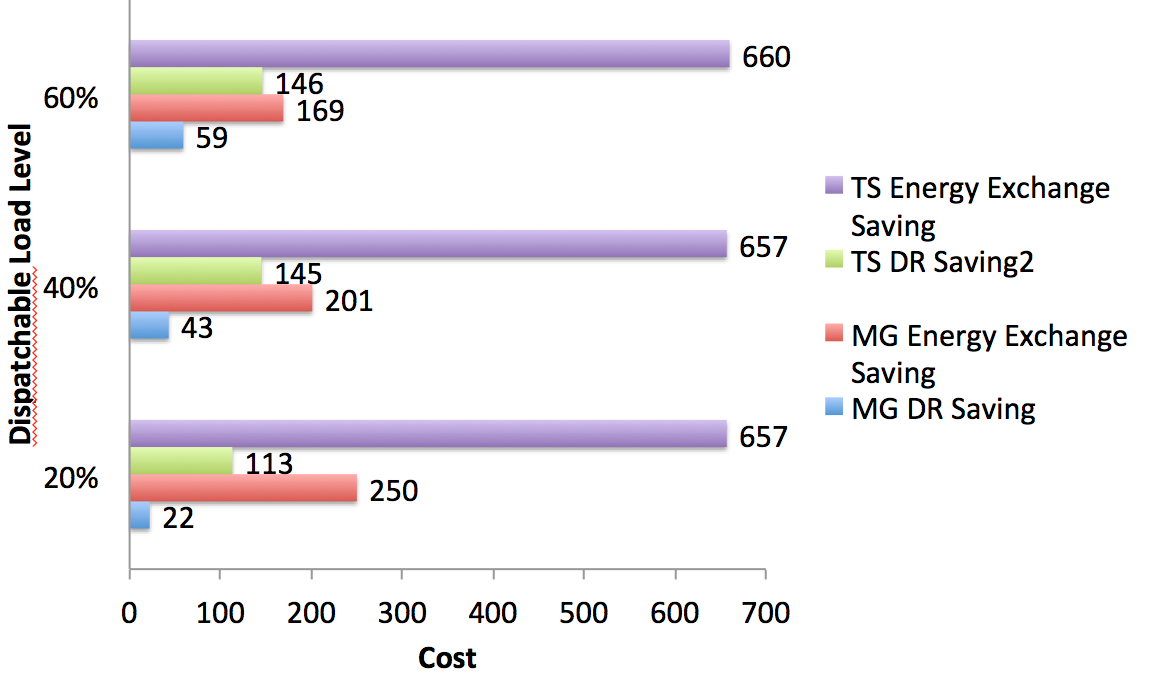
\includegraphics[scale=0.6]{pdsize2.png}
%%\caption{TS and MG savings breakdown for different MG DL levels}
%%\label{pdsize2}
%%\end{figure}
%
%It is shown in Fig.\ref{pdsize} that the TS cost decreases with an increasing DL level as more wind forecast error is accounted by the cheaper MG DR. However that decrease is not significant. In contrast, the MG cost decreases significantly with the increasing DL level as the MG has more DR to sell and more load flexibility. Once again, the Coop framework enables mutual financial benefits from the reserve service and energy exchange and thus reduces the cost of the two systems. The savings breakdown in Fig.\ref{pdsize2} gives further insights about the co-optimization. The energy exchange saving of the TS stays more or less the same for different dispatchable load levels as the net energy exchange quantity with the TS is more or less the same among the three cases. On the contrary, the energy exchange savings for the MG decreases with an increasing dispatchable load level. That is because the cost increasing rate of the MG in the SA mode is great than that in the Coop mode with a decreasing dispatchable load level as the Coop mode enables cost saving from energy exchange. The DR savings for both systems increase with an increasing dispatchable load level as a higher level enables more DR service. However, the DR saving for the TS from 40\% to 60\% DL does not increase much as the marginal cost benefit for that additional DR is very small.
%
%\subsubsection{Wind farm and MG locations on transmission and MG cost}
%With 10\% WP, a 25MW MG with 50\% DL system configuration, the location of the wind farm and the MG does not make a difference in terms of the system operation cost as this WP does not cause congestion anywhere in the system. However it is possible that a higher WP at certain buses could cause congestion and significantly increases the system operating cost, which is a well-known fact in the power systems. The way to wisely position the MG to deal with the congestion and reduce the system cost is discussed in \cite{liu2016quantifying}.

%\section{Concluding Remarks}\label{sec:Conclude}
%\input{conclusion}
\section{Appendix}\label{sec:Appendix}
%!TEX root = Journal.tex
\subsection{Big-M Method}
The complementary conditions are set of constraints with the following format:\\
\begin{align}
\lambda_i*g_i(x,y) =0 \nonumber
\end{align}
Specifically, given a sufficiently large positive value $M_i$ and binary value $\phi_i$, the complementary conditions could be reformulated as below:
\begin{align}
&-(1-\phi_i)*M_i\leq g_i(x,y)\nonumber\\
&\lambda_i\leq\phi_i*M_i\nonumber
\end{align}

For a detailed treatment of the Big-M method, please refer to \cite{winston2003introduction}.

%\subsection{Mccormick Envelope}
%For a toy optimization problem of the following format:\\
%\begin{align}
%\text{min } Z = x*y\\ \nonumber
%\underline{x} \leq x \leq \overline{x} \nonumber\\
%\underline{y} \leq y \leq \overline{y} \nonumber
%\end{align}
%The problem could be reformulated by introducing a new variable $w=x*y$ as follow:\\
%\begin{align}
%\text{min } Z = w\\ \nonumber
%w \geq \overline{x} *y +x*\overline{y} -\overline{x} *\overline{y} \nonumber\\  
%w \geq \underline{x} *y +x*\underline{y} -\underline{x} *\underline{y} \nonumber\\  
%w \leq \overline{x} *y +x*\underline{y} -\overline{x} *\underline{y} \nonumber\\
%w \leq \underline{x} *y +x*\overline{y} -\underline{x} *\overline{y} \nonumber\\
%\underline{x} \leq x \leq \overline{x} \nonumber\\
%\underline{y} \leq y \leq \overline{y} \nonumber
%\end{align}
%For a detailed treatment of the Big-M method, please refer to \cite{castro2015tightening}.

\subsection{Microgrid Parameters}
The parameter values for a 25 MW MG are listed in the table below.

\begin{table}[h]
\centering
\begin{tabular}{ |c|c|c| } 
 \hline
Parameters & Values  \\ 
 \hline
$\underline{L}^d_{t}$ & 6.6MW  \\ 
 \hline
$\overline{L}^d_{t}$ & 12MW  \\ 
 \hline
$L^i_{t}$ & 12MW  \\ 
 \hline
$\overline{B}$ & 10MW  \\ 
 \hline
$\underline{B}$ & 0MW \\ 
 \hline
$C^b$ & \$0.1/MW  \\ 
 \hline
$C^{m1}_t$ & \$4/MW  \\ 
 \hline
$C^{m2}_t$ & \$0.07/MW  \\ 
 \hline
 $C^{dr1}_t$ & \$0.4/MW  \\ 
 \hline
$C^{dr2}_t$ & \$0.3/MW  \\ 
 \hline
$C^d_t$ & \$6/MW  \\ 
 \hline
 $\overline P^d_t$ & \$1/MW  \\ 
 \hline
$\overline P^m$ & 25MW  \\ 
 \hline
$\underline P^m$ & 0MW  \\ 
 \hline
$\underline P^b$ & -5MW  \\ 
 \hline
$\overline P^b$ & 5MW  \\ 
 \hline
\end{tabular}
\caption{ MG parameter values}
 \label{wdlevel}
\end{table} 
% curtailment policy could be extracted from the 




%\IEEEtriggercmd{\enlargethispage{-0.52in}}
%\IEEEtriggeratref{1}
\clearpage
%%%%%%%%%%%%%%%%%%%%%%%%%%%%%%%%%%%%%%%%%%%%%%
 \bibliographystyle{IEEEtran}
 \bibliography{HICSS51}
%%%%%%%%%%%%%%%%%%%%%%%%%%%%%%%%%%%%%%%%%%%%%%


\end{document}




